\documentclass[tikz,border=2]{standalone}
\usetikzlibrary{shadows,arrows,shapes,positioning,calc,backgrounds,fit}
% Define the layers to draw the diagram
%
\begin{document}
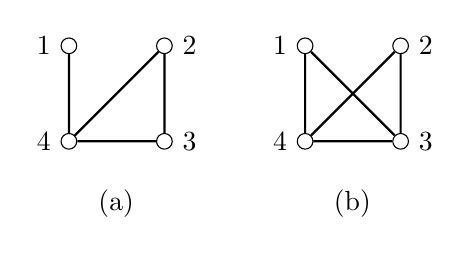
\begin{tikzpicture}
[node distance=1cm,
vertex/.style={shape=circle,draw=black,inner sep=2pt},
myedge/.style={thick}]

\node (v11) [vertex,label=left:$1$] at (0,0) {};
\node (v21) [vertex,right=of v11,label=right:$2$] {};
\node (v31) [vertex,below=of v21,label=right:$3$] {};
\node (v41) [vertex,below=of v11,label=left:$4$] {};
\draw[myedge] (v11) -- (v41) -- (v31) -- (v21) -- (v41);
\node at (0.6,-2) {(a)};

\node (v12) [vertex,label=left:$1$] at (3,0) {};
\node (v22) [vertex,right=of v12,label=right:$2$] {};
\node (v32) [vertex,below=of v22,label=right:$3$] {};
\node (v42) [vertex,below=of v12,label=left:$4$] {};
\draw[myedge] (v12) -- (v42) -- (v32) -- (v22) -- (v42);
\draw[myedge] (v12) -- (v32);
\node at (3.6,-2) {(b)};

%\node (v13) [vertex,label=left:$1$] at (6,0) {};
%\node (v23) [vertex,right=of v13,label=right:$2$] {};
%\node (v33) [vertex,below=of v23,label=right:$3$] {};
%\node (v43) [vertex,below=of v13,label=left:$4$] {};
%\draw[myedge] (v13) -- (v43) -- (v33) -- (v23) -- (v43);
%\draw[myedge] (v23) -- (v13) -- (v33);
%\node at (6.6,-2) {(3)};

%\node (v14) [vertex,label=left:$1$] at (9,0) {};
%\node (v24) [vertex,right=of v14,label=right:$2$] {};
%\node (v34) [vertex,below=of v24,label=right:$3$] {};
%\node (v44) [vertex,below=of v14,label=left:$4$] {};
%\draw[myedge] (v14) -- (v44) -- (v34) -- (v24) -- (v44);
%\draw[myedge] (v24) -- (v14) -- (v34);
%\node at (9.6,-2) {(4)};

\end{tikzpicture}
{}
\end{document}
